\documentclass[10pt]{beamer}
\usetheme[ ]{Feather}
  

%-------------------------------------------------------
% INCLUDE PACKAGES
%-------------------------------------------------------

\usepackage[utf8]{inputenc}
\usepackage[french]{babel}
\usepackage[T1]{fontenc}
\usepackage{helvet}
\usepackage{multirow}

%-------------------------------------------------------
% DEFFINING AND REDEFINING COMMANDS
%-------------------------------------------------------

% colored hyperlinks
\newcommand{\chref}[2]{
  \href{#1}{{\usebeamercolor[bg]{Feather}#2}}
}

%-------------------------------------------------------
% INFORMATION IN THE TITLE PAGE
%-------------------------------------------------------

\title[] % [] is optional - is placed on the bottom of the sidebar on every slide
{ % is placed on the title page
      \textbf{Indexation d'un fichier XML}
}

\subtitle[Master ISI1]
{
%      \textbf{v. 1.0.0}
}

\author[Amri Habiba Sabri Zineb ]
{     Amri Habiba  \\
      {\ttfamily Sabri Zineb}
}

\institute[]
{
      Departement Informatique\\
      Université Caddi Ayad, Faculté de Science Smlalia\\
  
  %there must be an empty line above this line - otherwise some unwanted space is added between the university and the country (I do not know why;( )
}

\date{\today}

%-------------------------------------------------------
% THE BODY OF THE PRESENTATION
%-------------------------------------------------------

\begin{document}

%-------------------------------------------------------
% THE TITLEPAGE
%-------------------------------------------------------

{\1% % this is the name of the PDF file for the background
\begin{frame}[plain,noframenumbering] % the plain option removes the header from the title page, noframenumbering removes the numbering of this frame only
  \titlepage % call the title page information from above
\end{frame}}


\begin{frame}{Plan}{}
\tableofcontents
\end{frame}

%-------------------------------------------------------
\section{Introduction}
%-------------------------------------------------------


\subsection{Problématique}
\begin{frame}{Introduction}{Problématique}
%-------------------------------------------------------

\begin{figure}[t]
    
    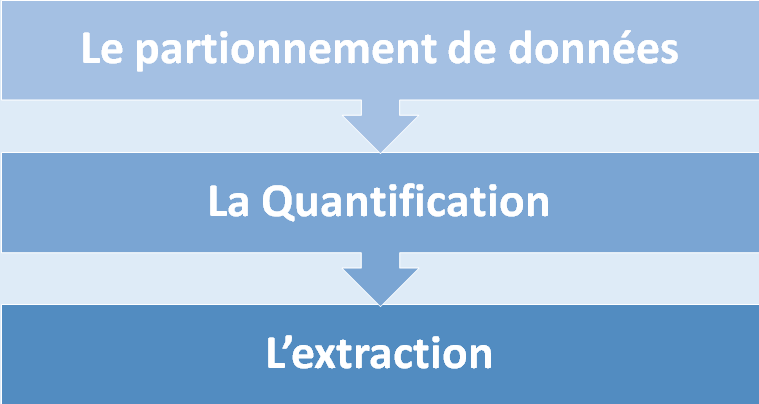
\includegraphics[height=\dimexpr10\textheight/16\relax]{reco_exst_1}
    
  \end{figure}
\end{frame}


%-------------------------------------------------------
\subsection{Solution}
%-------------------------------------------------------


\begin{frame}{Introduction}{Solution}
\begin{figure}[t]
    \centering
    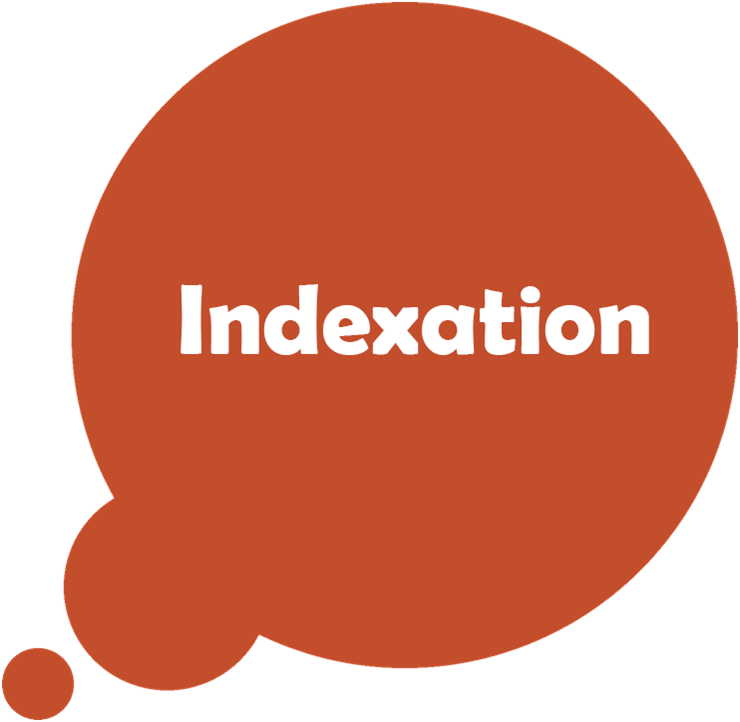
\includegraphics[height=\dimexpr10\textheight/16\relax]{22}
   
  \end{figure}
\end{frame}


%-------------------------------------------------------

\begin{frame}{Introduction}{Solution}
%-------------------------------------------------------
\begin{figure}[t]
    \centering
    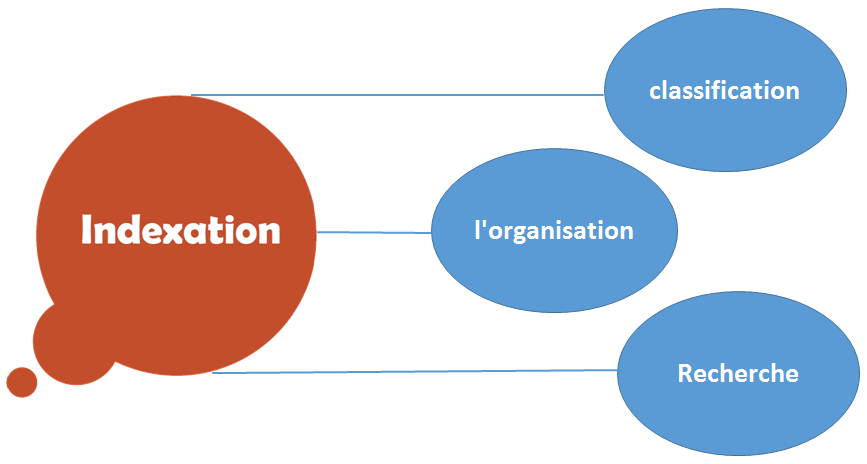
\includegraphics[height=\dimexpr10\textheight/16\relax]{Untitled}
  
  \end{figure}
\end{frame}
\section{Outils}
%-------------------------------------------------------

\begin{frame}{Outils}{Lucene}
%-------------------------------------------------------
\begin{figure}[t]
    \centering
    
\includegraphics[height=\dimexpr10\textheight/16\relax]{lucene}
   
  \end{figure}
\end{frame}
\begin{frame}{Outils}
%-------------------------------------------------------

\begin{block}{Historique}
Lucene est d'abord mis en téléchargement par Doug Cutting sur le site SourceForge.net en mars 2000. Son transfert vers Apache Jakarta est annoncé en octobre 2001.
\end{block}

\begin{block}{Lucene}Lucene est une bibliothèque open source écrite en Java qui permet d'indexer et de chercher du texte. Il est utilisé dans certains moteurs de recherche.
\end{block}
\end{frame}

\begin{frame}{Outils}
\begin{block}{Apache Lucene en bref}
\begin{itemize}
\item Langage :Java 
\item Iterfaces Disponibles : Lucene a été porté dans de multiples langages,dont C, C++, Python, Ruby, Perl, Lisp, PHP,etc
\item Plateformes supportées : Toute plateforme disposant d'une machine virtuelle Oracle Java ou OpenJDK en version 7 et supérieures 
\item Licence : Apache 2.0 
\item Principaux utilisateurs : Airbus, Apple, Disney, IBM, LinkedIn, Twitter (dans une version modifiée) 


\end{itemize}
\begin{flushright}
Source : JDN
\end{flushright}


\end{block}
\end{frame}

\section{Objectifs}
\begin{frame}{Objectifs}
\begin{figure}[t]
    \centering
    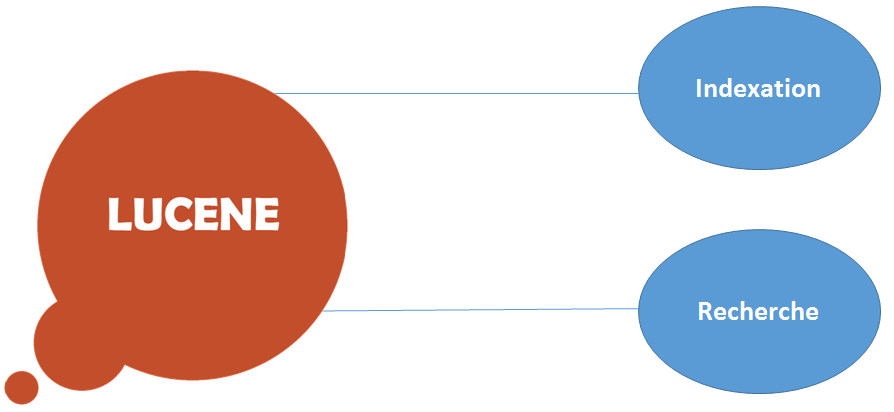
\includegraphics[height=\dimexpr9\textheight/16\relax]{33}
  \end{figure}
\end{frame}



%-------------------------------------------------------
\section{Démonstration}
\begin{frame}{Démonstration}
%-------------------------------------------------------

\begin{figure}[t]
    \centering
    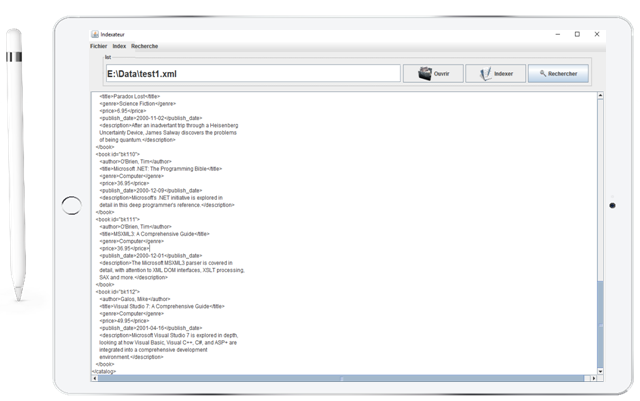
\includegraphics[height=\dimexpr10\textheight/16\relax]{image}
  \end{figure}
\end{frame}
%-------------------------------------------------------
\section{Conclusion}

\begin{frame}{Conclusion}{Points forts}
%-------------------------------------------------------

\begin{itemize}

\item Forte communauté, avec des mises à jour fréquentes 
\item Faible empreinte mémoire, de nombreux projets open source qui viennent compléter le moteur lui-même
\item Lien vers le Big Data (notamment le projet Blur qui tisse un lien entre Lucene et Hadoop)

\end{itemize}

\end{frame}

%-------------------------------------------------------
\section{References}
\begin{frame}{References}
%-------------------------------------------------------

\bibliographystyle{abbrv}
%\bibliography{sigproc}

\begin{thebibliography}{1}

\bibitem{rankAggregation}
https://fr.wikipedia.org/wiki/Lucene

\bibitem{bundleReco}
http://lucene.apache.org/
\bibitem{bundleReco}
http://www.torrefacteurjava.fr/content/
\bibitem{bundleReco}
https://wiki.apache.org/lucene-java/
\bibitem{bundleReco}
http://www.w3ii.com/fr/lucene/default.html
\bibitem{bundleReco}
https://wiki.apache.org/lucene-java/
\bibitem{bundleReco}
http://www.w3ii.com/fr/lucene/default.html
\bibitem{bundleReco}
http://blog.soat.fr/2010/09/comment-utiliser-lucene-dans-vos-applications/
\bibitem{bundleReco}
http://www.journaldunet.com/solutions/saas-logiciel/5-moteurs-de-recherche-open-source/apache-lucene.shtml
\bibitem{simrank}
M. McCandless, E. Hatcher, and O. Gospodnetić.
\newblock Livre:  {\em Lucene In Action}
\end{thebibliography}
\end{frame}


{\1
\begin{frame}[plain,noframenumbering]
  \finalpage{Merci pour votre attention ;)! Questions?}
\end{frame}}

\end{document}